\documentclass[a4paper,english,russian]{G2-105}
\usepackage[T1]{fontenc}
\usepackage{listings}
\usepackage{graphicx}
\usepackage{longtable}
\usepackage{booktabs}
\usepackage{standalone}
\usepackage{newclude}
\usepackage[final]{pdfpages}
\usepackage{multirow}
\usepackage{sansmath} % Enables turning on sans-serif math mode, and using other environments
\sansmath % Enable sans-serif math for rest of document
\usepackage[math]{blindtext}

%\usepackage[utf8]{luainputenc}
\VSTUSetDocumentNumbersPrefix{}
\VSTUSetDocumentCode{ВРБ-40 461 806-10.27-10-17.81}
\VSTUSetDocumentTypeDative{выпускной работе бакалавра}
\VSTUSetDocumentTypeGenitive{выпускную работу бакалавра}
\VSTUSetInitialData{задание, выданное научным руководителем с кафедры САПРиПК,
утвержденное приказом ректора}

\VSTUSetPZContents{
    \begin{VSTUList}
    \ulitem{Введение}
    \ulitem{1 Обзор фреймворков машинного обучения}
    \ulitem{Выводы}
    \ulitem{2 Используемые алгоритмы и модели}
    \ulitem{Выводы}
    \ulitem{3 Проектирование системы}
    \ulitem{Заключение}
    \ulitem{Список использованных источников}
    \ulitem{Приложение A - Техническое задание}
    \ulitem{Приложение Б - Архитектура сверточной нейронной сети Tiny YOLO}
    \end{VSTUList}
}

\VSTUSetPZGraphics{
    \begin{VSTUNumberedList}
    \ulitem{1: Название работы}
    \ulitem{2: Проблема}
    \ulitem{3: Цель и задачи}
    \ulitem{4: Аналоги}
    \ulitem{5: Требования}
    \ulitem{6: Проектирование. Use Case Diagram}
    \ulitem{7: Проектирование. Activity Diagram}
    \ulitem{8-9: Реализация}
    \ulitem{10: Выводы}
    \end{VSTUNumberedList}
}


\begin{document}
\VSTUSetOrder{1548-ст}{1}{ноября}{2017}
\VSTUSetFaculty{Электроники и вычислительной техники}
\VSTUSetDepartment{Системы автоматизированного проектирования и ПК}
\VSTUSetDepartmentCode{10.27}
\VSTUSetDirection{230100 Информатика и вычислительная техника}
\VSTUSetHeadOfDepartment{и.о. зав. кафедрой САПРиПК}{д.т.н., проф.}{М. В. Щербаков}{Щербаков Максим Владимирович}
\VSTUSetDirector{доцент каф. САПРиПК}{к.т.н.}{А. В. Катаев}{Катаев Александр Вадимович}
\VSTUSetFacilityExpert{}{}{}{}
\VSTUSetStandardsAdviser{доцент каф. САПРиПК}{к.т.н.}{О. А. Шабалина}{Шабалина Ольга Аркадьевна}
\VSTUSetStudent{ИВТ-461}{Т. А. Мельников}{Мельников Тимофей Алексеевич}
\VSTUSetTitle{Портирование сверточной нейросети на ARM архитектуру с ограниченными вычислительными ресурсами и ресурсами памяти}
\VSTUSetTitleEng{Porting a convolutional neural network on the ARM architecture with the limited computing resources and limited memory resources}
%\VSTUAddChapterWordToTOC % обязательно для ПЗ в магистерских диссертациях
\VSTUInitializePZ
\abstract{Аннотация}
\par Документ представляет собой пояснительную записку к выпускной работе бакалавра на тему «Портирование сверточной нейросети на ARM архитектуру с ограниченными вычислительными ресурсами и ресурсами памяти», выполненную студентом группы ИВТ-461, Мельниковым Тимофеем Алексеевичем.
\par В данной работе рассмотрена возможность реализации алгоритмов машинного обучения, в частности прямой проход сверточной нейронной сети, на устройстве с ограниченными вычислительными ресурсами и ресурсами памяти.
\par Объём пояснительной записки составил \totalpages~страниц и включает \totalfigures~рисунков и \totaltables~таблицы. 
%\newpage
\newpage

\abstract{Annotation} \ttl
\par This document provides an explanatory note to the final work on the bachelor: «Porting a convolutional neural network on the ARM architecture with the limited computing resources and limited memory resources», developed by Melnikov Timofey Alekseyevich, IVT-461.
\par The possibility of implementing machine learning algorithms on a device with limited computing resources and memory resources is considered in this final. In particular,  forward function of a convolutional neural network.

\tableofcontents
\newpage

\starchapter{Введение} \ttl
\par Задачи обработки и анализа аналоговой информации являюся одиними из самых сложных в IT-индустрии. Долгое
время такие задачи решались алгоритмами, которые требовали огромных аппаратных ресурсов при малой точности результата. На протяжении последних десяти лет стремительно растет и развивается прикладная область математики цель которой, изучение и развитие искусственных нейронных сетей \cite{1}. Актуальность разработок и исследований в данной области оправдывается применением НС в различных сферах деятельности. Это автоматизация процессов анализа объектов, образов, уневерсализация управления, прогнозирование, создание экспертных систем, анализ неформализованной информации и многое другое. В частности, в данной дипломной работе используются нейронные сети для классификации и обнаружения объектов на изображении. 
\par Наиболее существенным недостатком НС является их требовательность к вычислительным ресурсам и ресурсам памяти. Частично данная проблема решается использованием сверточных нейронных сетей, которые, в виду особенностям логики работы, позволяют в разы сократить ресурсы потребляемые нейронной сетью \cite{2}.
\par Однако, не только искусственные нейронные сети являются трендом IT-идустрии, активно развивается коцепция интернета вещей. Диапазон встраиваемых технологий простирается от концепции умных зданий до промышленной консолидации. Совмещение встраиваемых систем и искусственных нейронных сетей позволяет иначе взглянуть на решение нетревиальных задач, таких как автономное управление автомобилем \cite{3}.
\par В связи с вышесказанным целью данной дипломной работы является внедрение фреймворка машинного обучения на ARM-устройство и последующая оптимизация его работы. На основе проделанной работы необходимо сделать вывод о эффективности и рентабельности данного решения. 
\par Для достижения поставленной цели необходимо решить следующие задачи:
\begin{itemize}
\item Изучить фреймворки глубокого машинного обучения;
\item Разработать консольное приложение для реализации прямого прохода нейронной сети;
\item Оптимизировать использование оперативной памяти и реализовать загрузку весов по мере использования;
\item Разработать клиент-серверное приложение, демонстрирующее результат работы.
\end{itemize}
\par В первом разделе пояснительной записки описаны фрейворки машинного обучения. Далее приведено обоснование выбора фреймворка darknet.
\par Во втором разделе описаны используемые модели нейронных сетей и алгоритм прямого прохода.
\par Третей раздел посвящен разворачиванию фреймворка на ARM-устройсто и оптимизации работы алгоритма прямого прохода. Так же описана разработка клиент-серверной части для визуализации работы приложения. 
\newpage




\chapter{Обзор технологий и фреймворков машинного обучения}


\section{Исскуственные нейронные сети}
\subsection{Нейронные сети: основные положения}
\par Основой любой нейронной сети являются однотипные, простые элементы, которые представляют собой упрощенную модель нейронов мозга. Далее по тексту термин “нейрон” используется для определения ячейки нейронной сети --- искусственного нейрона. В соответствии с клетками головного мозга, которые могут быть возбужденными или заторможенными, нейрон характеризуется состоянием в момент прохода нейронной сети. Каждый нейрон обладает набором синапсов и одним аксоном. Синапсы являются однонаправленными связями, которые связывают конкретный нейрон с выходами группы других нейронов. В свою очередь, аксон передает сигнал нейрона на синапсы нейронов, расположенных на следующем слое. На рисунке ~\ref{neuron} представлен общий вид нейрона. Каждый синапс описывается величиной синаптической связи, иными словами, синапсы характеризуются весом $w_i$, который является аналогом электрической проводимости в клетках мозга \cite{4}.
\begin{figure}
	\begin{center}
    		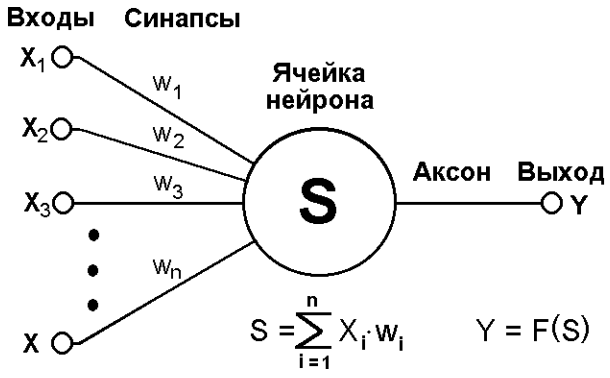
\includegraphics[width=0.6\linewidth]{neuron.png}
    		\caption{Исскуственный нейрон}
		\label{neuron}
	\end{center}
\end{figure}
\par Теоретически количество слоев (глубина) и количество нейронов в них (высота), используемых в НС, не ограниченно, но фактически ограничения накладывают вычислительные мощности устройства, на котором выполняется обработка НС. Но чем сложнее НС, тем масштабнее задачи она может решить. 
\par Структура НС зависит от сложности задачи. Оптимальные конфигурации для некоторых типов задачи уже реализованны и описаны, например в \cite{5}. Если же задача не является типовой, то разработчик самостоятельно генерирует модель, в зависимости от сложности задачи, размера обучающей выборки и вычислительных ресурсов. При этом необходимо учитывать основопологающие принципы: качество модели напрямую зависит от количества нейронов сети, плотности связей между ними и количеством слоев; сложность алгоритмов функционирование сети (например, введение нескольких типов синапрос, использование непороговых активационных функций) влиет на производительность НС. Задача поиска оптимальной конфигурации для той или иной задачи является отдельным направлением нейрокомпьютерной науки. Синтез нейронной сети напряму зависит от типа решаемой задачи, поэтому список подробных рекомендаций составить затруднительно. В большинстве случаев оптимальный вариант выбирается эмпирическим методом \cite{6}.
\par Очевидно, что функционирование нейронной сети напрямую зависит от величины синаптических связей между нейронами. Поэтому, после нахождения конфигурации нейронной сети, разработчик должен найти оптимальные значения всех переменных весовых коэффициентов (некоторые веса могут быть постоянными).
\par Описанный процесс называется обучений нейронной сети, он является ключевым при сознании НС. От того, насколько хорошо он будет выполнен, зависит качество решений поставленных задачь перед нейронных сетей. На этапе обучение кроме качества поиска весов важное место занимает такой параметр как время обучения. Эти два параметра обратно пропорциональны: чем лучше подобраны веса, тем больше затрачено времени на обучение \cite{7}.


\subsection{Сверточные нейронные сети}
\par Сверточные нейронные сети имеют схожие характеристики с обычными нейронными сетями. Они состоят из нейронов, которые имеют обучаемые веса. Каждый нейрон преобразует входные данные в выходной сигнал, который, возможно, будет изменен нелинейностью. Каждая такая сеть имеет функцию потерь на последнем полносвязным слоем.
\par Изменения заключаются в том, что архитектура сверточных сетей построена на явном предположении, что входной слой представляет собой изображения. Это предположение вносит особые свойства в архитектуру сети. Функция прямого прохода становится более эффективной для реализации и значительно уменьшаются количество параметров сети \cite{8}.
\par Проблема регулярных нейронных сетей заключается в невозможности маштабирования. Например, в CIFAR-10 изображения имеют размер 32x32x3 (3 цветовых канала), поэтому каждый полносвязный нейрон в первом скрытом слое будет иметь 32 * 32 * 3 = 3072 веса. Данное количество весов является приемлемым для нейронной сети, но полносвязная структура не маштобируется. Например, если на вход подается изображение с размером 200x200x3, то каждый полносвязный нейрон будет иметь 200 * 200 * 3 = 120000 весов. Поэтому посносвязная структура сети использует огромные вычислительные ресурсы и ресурсы памяти. Большое количество параметров быстро приведет к переобучению.
\par В сверточных нейронных сетях учитывается тот факт, что на вход подается изображение, поэтому архитектура таких сетей оптимальней использует ресурсы памяти. В частности, в отличие от обычных сетей, сверточные используют нейроны, имеющие 3 измерения: ширина, высота, глубина (в CIFAR-10 ширина --- 32, высота --- 32, глубина --- 3). Нейроны в слое подключены только к малой области предыдущего слоя. На изображении ~\ref{convnn} показана структура сверточной нейронной сети. Красный слой на изображении представляет входной слой. Его ширина и высота будут размером изображения, а глубина равна 3-м \cite{9}.
\begin{figure}
    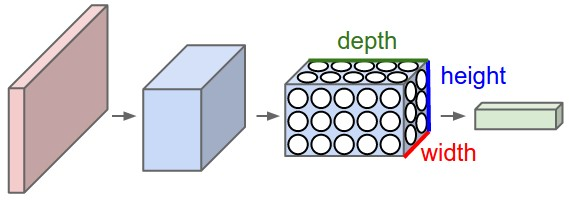
\includegraphics[width=\linewidth]{convnn.png}
    \caption{Структура сверточной нейронной сети}
	\label{convnn}
\end{figure}
\par Для построения архитектуры сверточной нейронной сети используются 3 основных типа своев: сверточный (convolution), слой объединения (pooling) и полносвязный. 
\par Для решение задачи классификации на размеченной базе CIFAR-10 может использоваться следующая архитектура:
\begin{itemize}
\item Входные данные [32x32x3]; 
\item Сверточный слой [32x32x12]; 
\item RELU-слой;
\item Объдиняющий слой [16x16x12];
\item Полносвязный слой [1x1x10].
\end{itemize}
\par Входной слой содержит исходные значения пикселей изображения. Сверточный слой вычисляет выходы нейронов, которые подключены к локальным областям на входе. Каждый нейрон имеет на выходе значение, вычесленное для небольшой области изображения. Это приводит к увеличению размерности слоя. В данном случае, слой будет иметь 12 фильтров, поэтому глубина слоя увеличится по отношению к входному слою. RELU-слой проводит активацию сверточного слоя. В таком слое применяется пороговая функция активации. В нашем случает используется функция $max(0, x)$. Размер слое остается неизменным. Объдиняющий слой выполняет операцию понижения дискретизации по пространственным измерениям (ширина, высота). Такое преобразование приводит к умешьшению размерности пространственных плоскостей. Полносвязный слой вычисляет оценки классов. Наждый из 10 значений соответствуют оценке класса, среди категорий CIFAR-10. Как и в случае с обычными нейронными сетями, каждый нейрон этого слоя связан со всеми нейроннами предыдущего слоя.
\par Таким образом сверточная нейронная сеть преобразует исходные значение пикселей изображения в итоговые оценки классов. В такой сети, некоторые слои содержат параметры, а другие нет. В частности, сверточный и полносвязный слой выполняют преобразования, которые являются функцией не только активации входного сигнала, но и параметров (веса, смещения нейронов). Объединяющий и RELU слои реализуют фиксированную функцию \cite{10}. 
\par В итоге, можно сделать следующие выводы:
\begin{itemize}
\item Архитектура сверточной нейронной сети в простейшем случае представляет собой список слоев, которые преобразуют изображения в выходные сигланы (например, вероятности классов изображений);
\item Существуют несколько разлизных типов слоев (Сверточный, объединяющий, RELU и полносвязный являются самыми популярными);
\item Каждый слой принивает 3-x мерный массив сигналов и преобразует его в выходной 3-х мерный массив сигналов через дифференцируемую функцию;
\item Каждый слой может иметь или не иметь параметров.
\end{itemize}
\par На рисунке ~\ref{convnet} показан результат работы сверточной нейронной сети. На данном изображении визуализированны выделенные признаки нейронной сетью на каждом из этапов прямго прохода.
\begin{figure}
    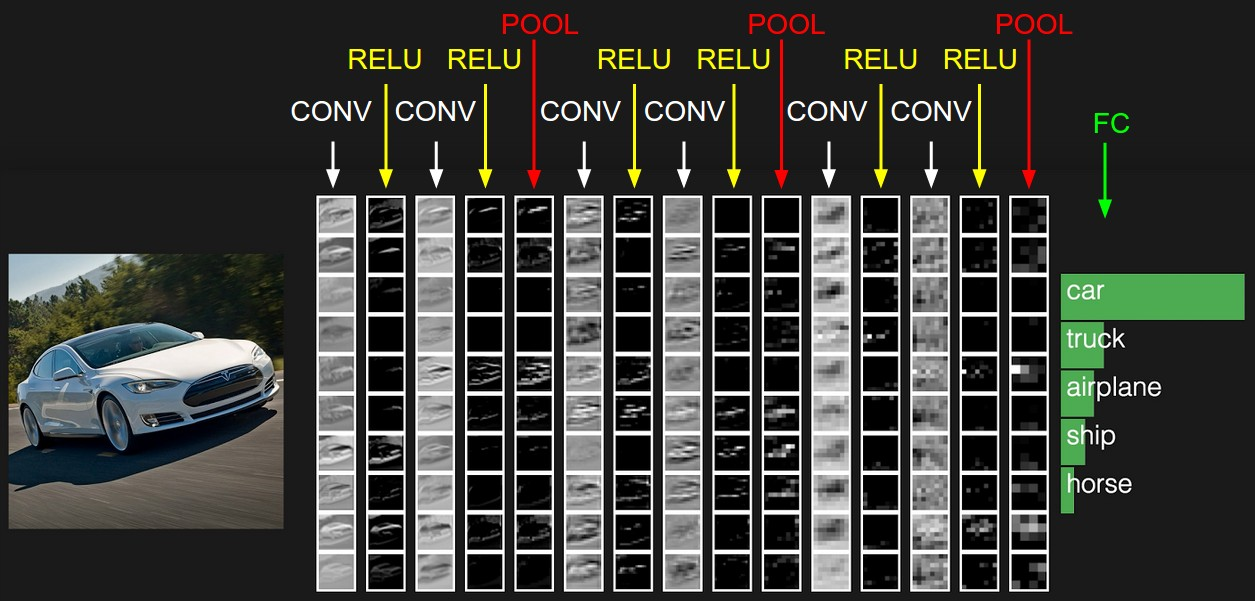
\includegraphics[width=\linewidth]{convnet.png}
    \caption{Визуализация работы сверточной нейронной сети}
	\label{convnet}
\end{figure}
\par Сверточный слой является основным стоительным блоком сверточной нейронной сети. На него затрачивается основная часть вычислительных ресурсов.
\par Для начала разберем сверточный слой без привязки к биологическому нейрону. Параметры слоя состоят из набора обучаемых фильтров. Фильтр является малым относительно входного пространства (по ширине и высоте), однако он проходит через всю глубину входного объема. Например, стандартный фильтр для первого сверточного слоя имеет размер 5х5х3 (Ширина и высота по 5 пикселей). Во время прямого прохода мы перемещаем фильтр по входному пространству и вычисляем свертку между локальными значениями входного пространства и значениями фильтра. При этом вычисляется двумерная карта активации, которая генерирует выход в каждом пространственном положении. На протяжении этого процесса сеть, активирует функции, которые представляют собой какую-либо визуальную информации. От различный линий на первом слое, и конкретные объекты изображения на конечном слое. В итоге, нейронная сеть, представленная выше, будет иметь 12 фильтров, каждый из который сгенерирует двумерную карту активаций.
\par При работе с высокоразмерными входами, такими как изображение, как было показано выше, не целесообразно связывать нейроны текущего слоя со всеми нейронами предыдущего слоя. Вместого этого в сверточных нейронных сетях каждый нейрон подключается только к локальной области входного объема. Пространственная протяженность этой связности является гирерпараметром, которые называется восприимчивым полем нейрона (размер фильтра). Важной особенносью является то, что соединения нейронов локальны в пространстве (по ширине и высоте), но всегда полны по всей глубине входного объема.
\par Например, если входным слоем является изображение 32x32x3 и размер фильра равен 5x5, то каждый нейрон в сверточном слое будет имет размер 5x5x3. В общей сложности 5*5*3 = 75 весов (и параметр смещения). 
\par На рисунке ~\ref{depthcol} показано пространственное подключение нейрона, но по полной глубине. 
\begin{figure}
    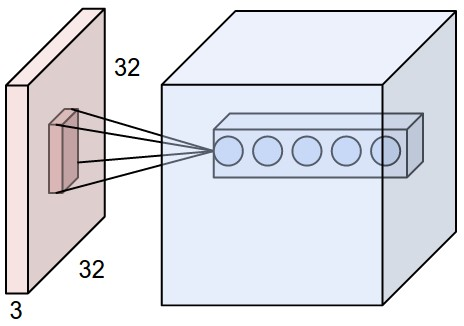
\includegraphics[width=0.5\linewidth]{depthcol.png}
    \caption{Визуализация свертчного слоя}
	\label{depthcol}
\end{figure}
\par Следующие параметры управляют размером выхода сверточного слоя:
\begin{itemize}
\item Глубина --- гиперпараметр, соответствующий числу фильтров. Каждый из фильтров обучается на поиск конкретного признака объекта;
\item Шаг --- величина на которорую сдвигается фильтр;
\item Нулевое заполнение --- размер размещений нулей вокруг границ входного пространства.
\end{itemize}
\ttl


\section{Обзор фреймворков машинного обучения}

\subsection{Фреймворк Caffe}
\par Caffe представляет собой фреймворк, разработанный учеными и практиками, с прозрачной и гибкой архитектурой для глубокого обучения и построения эталонных моделей. Фреймворк распространяется под BSD-лицензией и является c++ библиотекой. Так же реализованы python и MATLAB обертки для универсализации обучения и развертывания глубоких моделей. Caffe используется на промышленных компаниях и в медиацинтрах, обрабатывая 40 миллионов изображений в день на Titan GPU (примерно 2.5 милисекунд на изображение) \cite{11}.
\par Caffe сохраняет и передает данные в четырехмерных массивах, которые названы блобами. Блобы представляют унифицированный интерфейс для работы  памятью, содержащий пакеты ихображений (или других данных), параметров или обновлений параметров. Блобы скрывают вычислительные издержки смешанной работы CPU и GPU, выполняя синхронихацию по нере необходимости. Память выделяется по требованию (лениво), что позволяет эффективней ее использовать. Модели сохраняются как буфер, использующий протокол Google (Google Protocol Buffers), который имеет ряд достоинств: минимальный размер строки при сериализации, эффективная сериализация, высокая читабельность в текстовом виде и удобные интерфейсы работы на нескольких языках. Необходимые для обучения огромные массивы данных храняться в базах данныx LevelDB. Google Protocol Buffers и LevelDB обеспечивают пропускную способность в 150 Мб/с \cite{12}.
\par От других современных фреймворков глубокого обучения Caffe отличается следующими качествами:
\begin{itemize}
	\item Реализция полностью основана на C++, что облегчает интеграцию с встраиваемыми системами;
	\item CPU режим позволяет использовать фреймворк без специализированного GPU;
	\item Готовые модели позволяют не тратить время и ресурсы на обучение;
	\item Подробная документация для сериализации и использования моделей.
\end{itemize}

\subsection{Фреймворк Torch7}
\par Torch7 --- это универсальный математический фреймворк и библиотека машинного обучения, которая имеет оболочку для языка программирования Lua. Его цель --- предоставить гибкую среду для проектирования и обучения моделей глубокого обучения. Гибкость достигается с помощью Lua, так как он является очень легким скриптовым языком. Эффективная реализация низкоуровневых числовых процедур, используя OpenMP и CUDA, позволяет фрейморку достич выской производительности. Фреймворк имеет простой Lua-интерфейс, что позволяет легко подключать его к стороннему программному обеспечению.
\par Ключевой сущностью в Torch7 является класс Tensor, поставляемый автономной С-библиотекой Tensor. Данный класс расширяет базовый набор типов Lua, чтобы реализовать эффективную работу с многомерными массивами. Большинство пакетов Torch7 или сторонних пакетов, зависящих от Torch7, реализуют собственный класс Tensor для представления сигналов, изображений, видео и других объектов, что упрощает интегрирование различных библиотек. Библиотека Torch Tensor предоставляет множество классических операций (включая операции линейной алгебры), которые реализованны и оптимизированны на С, используются SSE интсрукции для Intel платформ. Опцианально можно использовать высокопроизовидельные реализации операций линейной алгебры в библиотеке BLAS. Так же данная библиотека поддерживает инструкции OpenMP и вычисления на CUDA GPU \cite{13}.
\par Структура фрейворка имеет три основных преимущества:
\begin{itemize}
\item она облегчает разработку численных методов;
\item фреймворк легко расширяем (включая использование сторонних библиотек);
\item высокая скорость работы фреймворка.
\end{itemize}

\subsection{Фреймворк Darknet}
\par Darknet один из немногих фреймворков машинного обучения, который не имеет обязательных зависимостей. Что позволяет быстро разворачивать его на встраиваемых системах. На ряду с встроенным функционалом, Darket поставляется с двумя опциональными зависимостями:
\begin{itemize}
\item OpenCV --- для предоставление более широкого спектра поддерживаемых форматов изображений;
\item CUDA --- для вычислений на GPU. 
\end{itemize}
\par Обе не являются обязательными для установки фреймворка \cite{14}.
\par Еще одним важным преимуществом фреймворка является независимость от архитектуры системы. Darknet полностью написан на C, что делает его универсальным, а его интеграцию в встраиваемы системы или в специализированное оборудование простой и понятной. 
\par В оригинальном виде фреймворк, поставляемый разработчиками, представляет консольное приложения для работы с нейронными сетями. С помощью него можно проектрировать, обучать, тестировать нейронные сети типовых топологий. В список функций так же входит визуализация модели классификации и обучение реккурентных моделей. Однако, конфигурация файлов исходных кодов спроектирована специально для предоставляения возможности компиляции необходимых модулей в библиотеку \cite{15}. Поэтому фреймворк можно встраивать как нативную библиотеку в любой пользовательский проект.
\par Основной структурой данных в фреймворке является динамический массив. Веса, изображения, строковые таблицы храняться в одномерном массие, который обернут в структуру соответствующего типа данных. Данный подход позволяет сократить издержки работы с памятью.

\section{Выводы}
\par Светрочные нейронные сети являются оптимальным решением для решения задачи детекции изображений на маломощном устройсте. Архитектура таких сетей позволяет сокращать изрержки на хранимые в памяти параметры.
\par Для использования сверточной нейронной сети на системе с ограниченными вычислительными ресурсами и ресурсами памяти необходимо, что бы фреймворк, поставляющий данные функции удовлетворял следующим условиям:
\begin{itemize}
\item высокопроизворительные вычисления;
\item оптимизированная работа с памятью;
\item минимальное число зависимостей.
\end{itemize}
\par Рассмотринные выше фреймворки, используя различные терхнологии и алгоритмы, обеспечивают высокую производительность своих реализаций. Caffe использует библиотеку BLAS (ATLAS, Intel MKL, OpenBLAS) для векторных и матричных вычислений, Lua в совокупности с технологиями SSE, OpenMP позволяют Torch показывать высокую скорость работы, бинаризация ядер в Darknet, позволяет использовать быстрые бинарные операции для расчетов.
\par Если говорить о оптимизации работы с памятью, то аппроксимация фильтров и входов в Darknet позволяет значительно уменьшить объем выделяемой памяти. На рисунке ~\ref{binary_conv} сравнение бинарной свертки и свертки с двойной точностью.
\begin{figure}
\begin{center}
    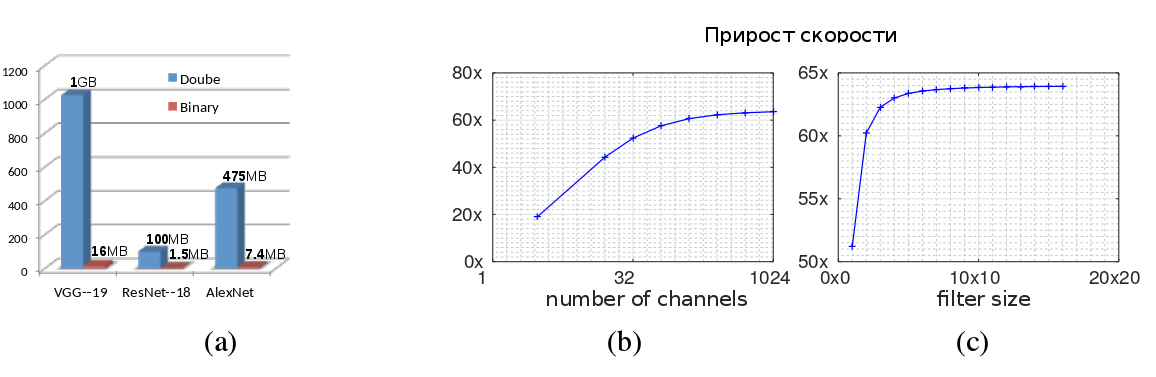
\includegraphics[width=0.55\paperheight]{binary_conv.png}
    \caption{Эффективность использования памяти и вычислений. a -- выделяемая память для весов различных архитектур, b --- ускорение в зависимости от числа каналов, c --- ускорение в зависимости от размера фильтра}
	\label{binary_conv}
\end{center}
\end{figure}
\par Caffe и Torch имеют достаточно большое количество зависимостей. Это объясняется желанием максимально ускорить процессы обучения и прохода нейронных сетей, однако наклабывает ограничения на срециализированное оборудование и оборудование с ограниченными запасами физической памяти.
\par Суммировав все показатели, можно сделать вывод, что Darknet является лучшим вариантов для разворачивания на маломощном ARM-устройтве.



\chapter{Используемые алгоритмы и модели}
\section{Обнаружение объектов с применем подхода YOLO}
\par Основная идея подхода YOLO стоиться на том, что обнаружение объекта определяется как проблема с одной регрессией, от пикселов изображения до координат ограничительной рамки и вероятностей классов. Такой подход позволяет за один проход сети определить, акие объекты присутствуют на изображении и где они находятся.
\par Архитектура YOLO представляет собой сверточную нейронную сеть, которая одновременно предсказывает локализацию объекта и класс найденного объекта. На рисунке ~\ref{yolo} показана схема работы детекции. Такая модель имеет несколько преимуществ над существующими решениями детекции объектов \cite{16}.
\begin{figure}
    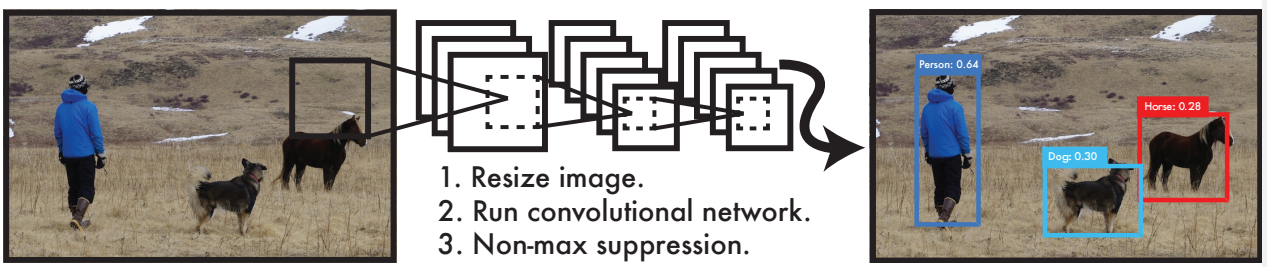
\includegraphics[width=\linewidth]{yolo.png}
    \caption{Система обнаружения YOLO}
	\label{yolo}
\end{figure}
\section{Архитектура сверточной сети YOLO}
\par Первые слои YOLO являеются сверточным и извлекают признаки объектов. Далее полносвязные слои прогнозируют вероятности и координаты объектов. Сеть имеет 24 сверточных слоя, за которыми следует 2 полносвязных слоя. Для уменьшения количества признаков используются сверточные слои с единичным фильтром. Полная сеть изображена на рисунке ~\ref{yolonet}.
\par Результатом сети является трехмерная матрица [7x7x30] содержащая информацию о ограничивающих блоках и вероятностей объекттов. 
\begin{figure}
	\begin{center}
    		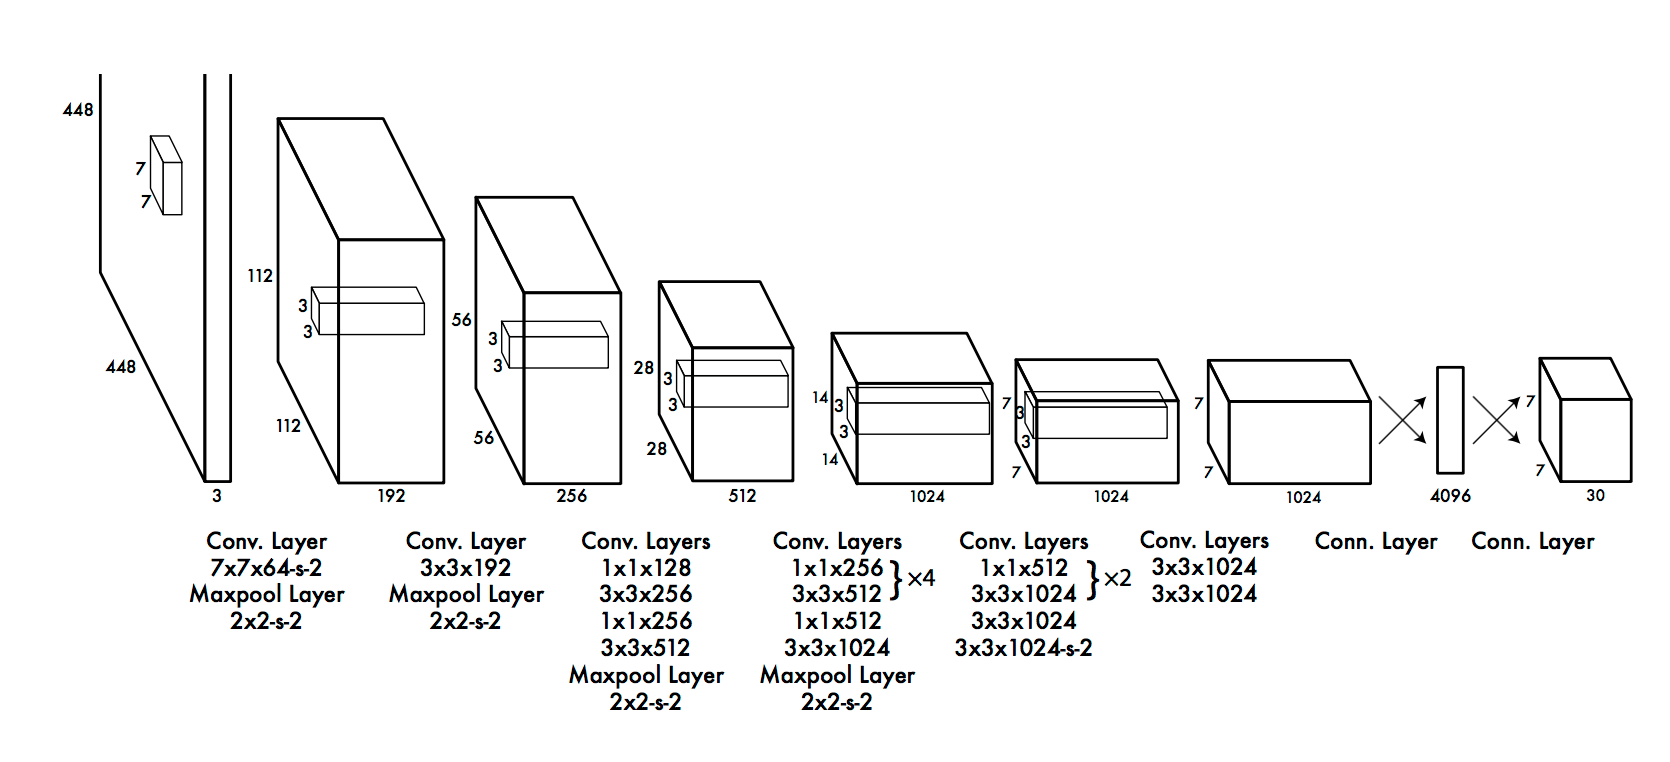
\includegraphics[width=\linewidth]{yolonet.png}
    		\caption{Архитектура нейросети YOLO}
		\label{yolonet}
	\end{center}
\end{figure}
\section{Алгоритм единого обнаружения}
\par Сеть YOLO делит входное изображение на сетку $SxS$. Если центр объекта попадает в ячейку сетки, эта ячейка сетки отвечает за обнаружение этого объекта.
\par Каждая ячейка сетки предсказывает $B$ ограничивающих рамок и оценки доверия для этих рамок. Эти оценки доверия отражают уверенность модели в том, что в рамке содержится объект. Формально, величина доверия определяется следующим образом:
\[
\ \hspace*{50mm} Pr(Object)*IOU_{pred}^{truth},  \ \hspace*{46mm} (14)
\]
\par где $Pr$ --- функция определяющая величину вероятности объекта, $IOU_{pred}^{truth}$ --- метрика пересечения между предсказанной локализацией и дейтвительным местоположением объекта \cite{17}.
\par Если объекта нет в данной ячейке, то оценка доверия должна быть равна нулю. В обратном случае, величина доверия равна пересечению между предстказанным местоположением и действительным местоположением объекта.
\par Каждый ограничивающий блок состоит из 5 прогнозов: $x, y, w, h$ и величина доверия. Координаты $(x, y)$ представляют собой центр блока относительно границ ячейки сетки. Ширина и высота предсказываются относительно всего изображения. Величина доверия представляет собой $IOU$ между предсказанным блоком и дейтвительным местоположением объекта.
\par Каждая ячейка сетки также пресказывает вероятности условного класса $C$. Эти вероятности обусловлены ячейкой сетки, содержащей объект \cite{18}. На рисукне ~\ref{yoloiter} изображена визуальная модель сети YOLO.
\par Во время тестирования условные вероятности классов и идивидуальные оценки доверия каждого блока. Эта оценка интерпритируется как вероятность того, что данный класс имеется в блоке и насколько предсказанный блок подходит для данного объекта. 
\par Суммировав вышесказанное, алгоритм работы YOLO выглядит следующим образом:
\begin{itemize}
\item Разделение изображения на сетку $SxS$;
\item Предсказание ограничивающих блоков $B$;
\item Предсказание классов $C$ для объектов в каждом блоке.
\end{itemize}
\begin{figure}
\begin{center}
    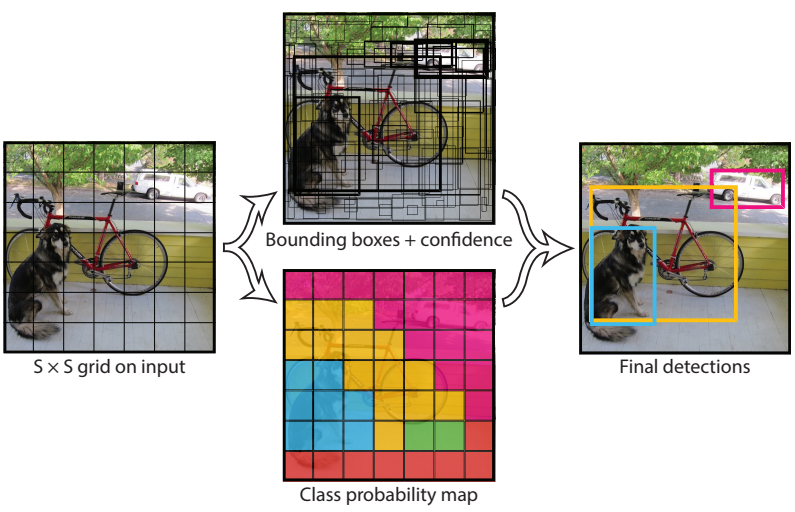
\includegraphics[width=0.7\linewidth]{yoloiter.png}
    \caption{Модель YOLO}
	\label{yoloiter}
\end{center}
\end{figure} 


\chapter{Проектирование системы}
\section{Архитектура системы}
\par Для полноценного функционирования система разделена на две части: клиентскую и серверную.
\par Клиентское приложение запускается на персональном компьютере и имеет GUI-интерфейс для общения c пользователем. В свою очередь серверное приложение, запускаемое на ARM-устройстве выполняет детекцию изображения и возвращает результат клиентскому приложению в виде размеченного изображения. Взаимодействие между клиенстким и серверным приложением осуществляется посредством TCP-сокетов.
\ttl
\subsection{Проектирование клиентского приложения}
\par Клиенское приложение необходимо для демонстрации вычислений сверточной нейронной сети, которая производится на ARM-устройстве. Оно представляет собой GUI-интерфейс, в котором пользователю предоставлются следующие возможности:
\begin{itemize}
\item Подключение к серверному приложению на ARM-устройстве;
\item Выбор изображения для детекции;
\item Запуск детекции на сервере;
\item Просмотр информации о этапах работы сервера;
\item Завершение работы серверного приложения.
\end{itemize}
\par На рисунке ~\ref{usecase} показана диаграмма вариантов использования клиенского приложения.
\par Что бы получать информацию о выполненных этапах детекции изображения на сервере, запущен дополнительный поток, который ожидает сообщения от сервера и выводит сообщение в текстовый браузер. 
\par В приложении 2 технического задания изображена диаграмма последовательности, на которой показана какая информация поступает от серверного приложения и в какой последовательности. 
\begin{figure}
    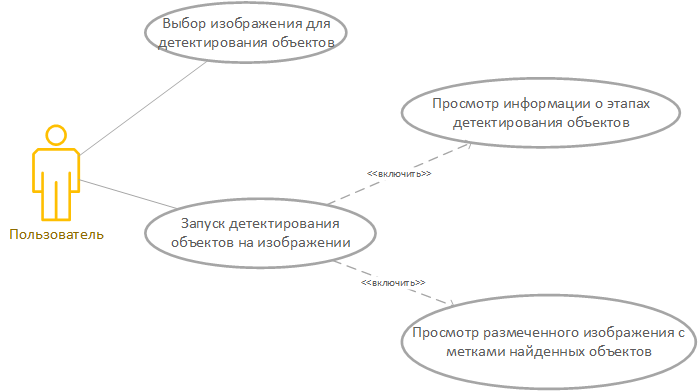
\includegraphics[scale = 0.7]{usecaseclient.png}
    \caption{Диаграмма вариантов использования клиенского приложения}
	\label{usecase}
\end{figure}
\ttl
\subsection{Проектирование серверного приложения}
\par Серверное приложение выполняется на ARM-устройстве. Оно реализует взаимодействие с клиентской частью, используя сокеты, и детекцию объектов на изображении с использованием API фреймворка darknet.
\par После подключения клиента, серверное приложения ожидает команды от клиентского приложения. Для запуска детекции изображения используетса команда "yolo". На рисунке ~\ref{state} изображена диаграмма деятельности, на которой показны функции, выполняемые серверным приложением в зависимости от поступившей команды клиетского приложения.
\par Завершение работы серверного приложение происходит при получении команды "exit". При этом серверное приложение закрывает дискриптор сокета, через который совершался обмен сообщениями.
\par Для обмена сообщениями между клиентским и серверным приложением реализован общий интерфейс передачи данных. В него входят функции приема и отправки текстовых сообщений и изображений.
\begin{figure}
    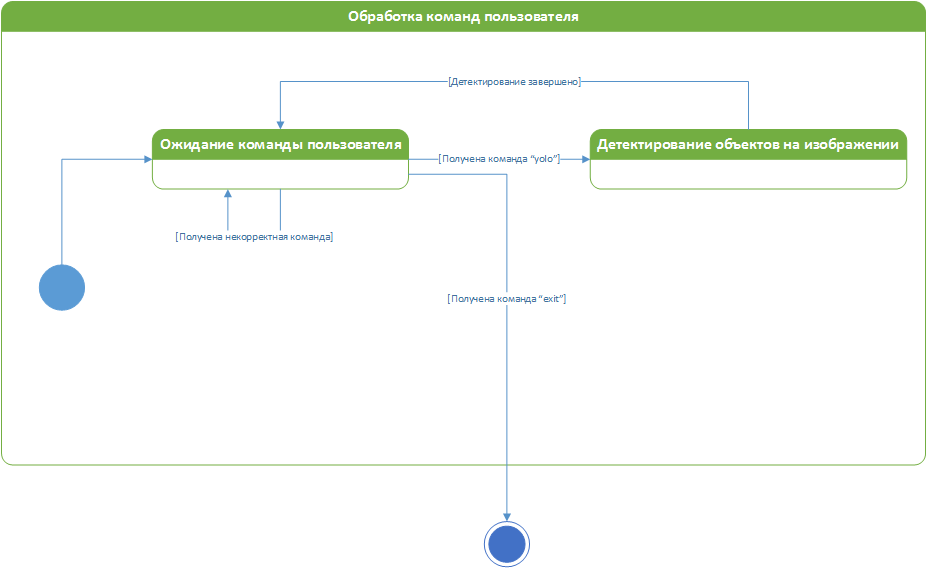
\includegraphics[width=\linewidth]{statediagramserver.png}
    \caption{Диаграмма деятельности серверного приложения}
	\label{state}
\end{figure}
\ttl
\subsection{Проектирование алгоритма прямого прохода сверточной нейронной сети}
\par Для реализации детектирование объектов на изображении используется API фреймворка darknet. В время работы детекции изображения серверное приложение отсылает клиенту информацию о пройденых этапах детекции. На рисунке ~\ref{activitydetector} изображена диаграмма последовательности, на которой показаны этапы детекции.
\par Для реализации прямого прохода нейронной сети использовались следующие функции, реализованные в фреймворке darknet:
\begin{itemize}
\item read\_data\_cfg --- осуществляет парсинг меток классов;
\item parse\_network\_cfg --- осуществляет парсинг конфигурации нейронной сети;
\item load\_weights --- сериализует веса нейронной сети;
\item load\_image\_color --- сериализует изображение для детекции;
\item network\_predict --- осуществляет прямой проход сериализованной нейронной сети;
\item draw\_detections --- осуществляет отрисовку ограничивающих объекты блоков и меток объектов.
\end{itemize}
\begin{figure}
    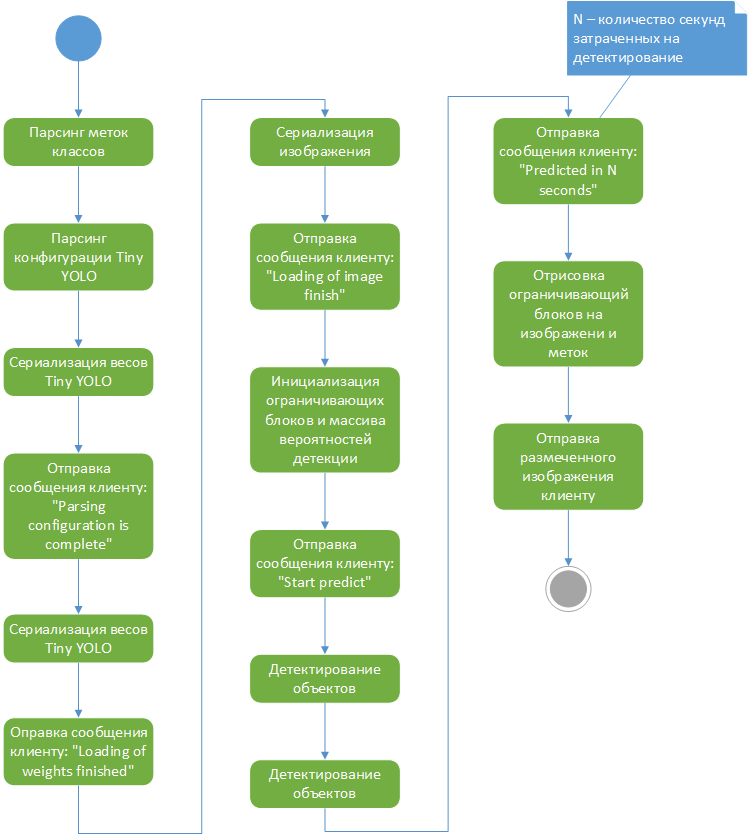
\includegraphics[width=0.8\linewidth]{activitydetector.png}
    \caption{Диаграмма последовательности алгоритма детектирования объектов}
	\label{activitydetector}
\end{figure}
\ttl
\section{Особенности реализации прямого прохода сверточной нейронной сети}
\par Для уменьшения затрат оперативной памяти при прямом проходе сверточной нейронной сети были произведены следущие мероприятия:
\begin{itemize}
\item Для реализации прямого прохода использовалась сверточная нейронная сеть Tiny YOLO;
\item После прохождения очередного слоя, память затраченная на его сереализацию очищается.
\end{itemize}
\par Архитектура сверточной нейронной сети Tiny YOLO в два раза меньше оригинальной сети YOLO. Соответсвенно занимаемая память на хранение сети уменьшилась в два раза. В приложении Б изображена архитектура Tiny YOLO. В таблице ~\ref{mbtable} показано количество занимаемой памяти сетью Tiny YOLO.
\begin{longtable}{|c|c|c|}
    \caption{Количество памяти, необходимое для сериализации весов Tiny YOLO} \label{mbtable} \\ \hline
    Имя слоя        & Размер слоя        &    Необходимое количество памяти, Мб \\ \hline \endhead
    Data           & 448x448x3 & 2,408 448 \\ \hline
    Conv1           & 224x224x64 & 12,845 056 \\ \hline
    Pool1           & 112x112x64 & 3,211 264 \\ \hline
    Conv2           & 112x112x192 & 9,633 792 \\ \hline
    Pool2           & 56x56x192 & 2,408 448 \\ \hline
    Conv3           & 56x56x128 & 1,605 632 \\ \hline
    Conv4           & 56x56x256 & 3,211 264 \\ \hline
    Conv5           & 56x56x256 & 3,211 264 \\ \hline
    Conv6           & 56x56x512 & 6,442 528 \\ \hline
    Conv7           & 28x28x256 & 0,802 816 \\ \hline
    Conv8           & 28x28x512 & 6,442 528 \\ \hline
    Conv9           & 28x28x256 & 0,802 816 \\ \hline
    Conv10           & 28x28x256 & 0,802 816 \\ \hline
    Conv11           & 28x28x256 & 0,802 816 \\ \hline
    Conv12           & 28x28x512 & 6,442 528 \\ \hline
    Conv13           & 28x28x256 & 0,802 816 \\ \hline
    Conv14           & 28x28x512 & 6,442 528 \\ \hline
    Conv15           & 28x28x512 & 6,442 528 \\ \hline
    Conv16           & 28x28x1024 & 3,211 264 \\ \hline
    Fc17           & 1x1x4096 & 0,016 384 \\ \hline
    Fc19           & 1x1x1470 & 0,005 880 \\
\end{longtable}
\par Суммарное количество памяти, необходимо для сериализации Tiny YOLO составляет 79,601 Мб. Это является приемлемыми затратами для мобильного пк C.H.I.P., который использользовался как ARM-устройство в данной работе. Однако, при прямом проходе каждого сверточного и объединяющего слоя генерируюся выходные сигналы. Поэтому, ресурсов C.H.I.P. не достаточно для осуществления прямого прохода. 
\par Для того, что бы оптимизировать работу с оперативной памятью при выгрузке слоев, был видоизменена функция прямого прохода нейрнных сетей в фрейворке darnket. Сам фремворк интегрируется посредством компилирования исходных файлов фреймворка в исполняемый файл серверного приложения. На рисунке ~\ref{alg} показаны различия между оригинальным алгоритмом прямого прохода и видоизмененным.
\begin{figure}
    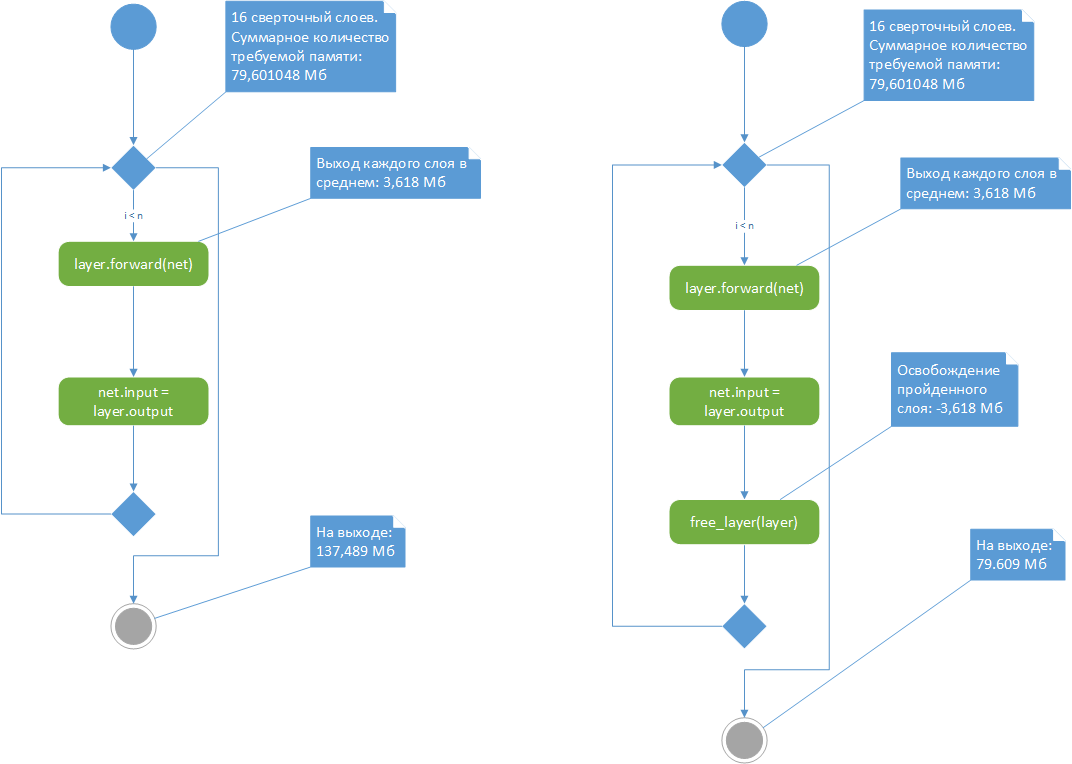
\includegraphics[width=\linewidth]{alg.png}
    \caption{Различие между оригинальным алгоритмом прямого прохода и видоизмененным}
	\label{alg}
\end{figure}
\par Удаление слоя после его прохода, позволяет уменьшать затраты оперативной памяти на каждой итераци вычислений и позволяет осуществлять детектирование объектов на маломощном устройстве C.H.I.P.
\ttl
\section{Требования к входным/выходным данным приложения}
\par Входными данными для клиентского приложения является изображения в форматах png и jpg.
\par Входными данными для серверного приложения являются файл с метками объектов, на детекцию которых обучена нейронная сеть формата data, конфигурационный файл формата cfg, изображение для детектирования в форматах png и jpg, веса нейронной сети в формате weights. В приложении 1 технического задания описаны форматы конфигурационных файлов нейронной сети.
\par Выходными данными системы является изображение с отображением меток детектированного изображения, данные о этапах детектирования и время выполнения детектирования.
\par На рисунке ~\ref{window} показан результат работы детектирования изображения. Слева на изображении отмечены прямоугольником обнаруженные объекты. Справа отображена информация об основных этапах детектирования данного изображения.
\begin{figure}
    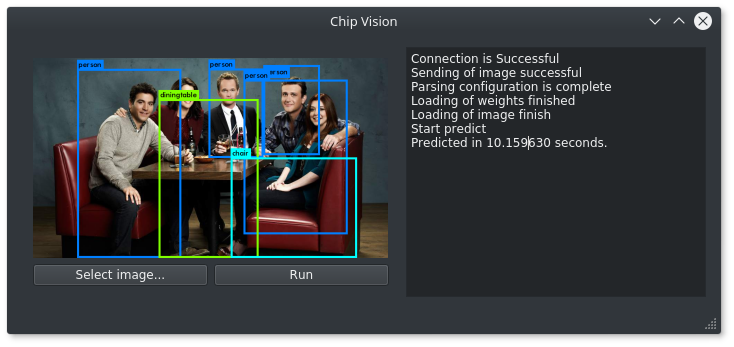
\includegraphics[width=\linewidth]{window.png}
    \caption{Пример работы детекции объектов}
	\label{window}
\end{figure}
\ttl
\section{Тестирование разработанного приложения}
\par На рисунке ~\ref{timedetection} показно время на детектирование изображений различных разрешений.
\begin{figure}
    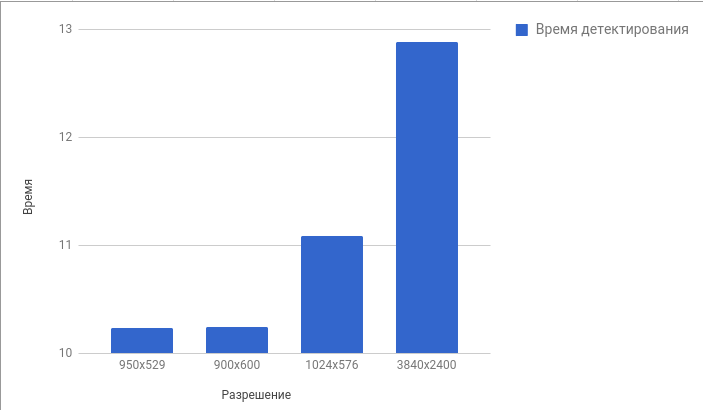
\includegraphics[width=0.6\linewidth]{timedetection.png}
    \caption{Диаграмма зависимости времени детекции от разрешения изображения}
	\label{timedetection}
\end{figure}
\par В среднем время на детектирование объектов состовляет 10,5 минут. С увеличением размерности изображение время увеличивается, это связано с затратами на изменение размера изображения.

\newpage
\starchapter{Заключение}
\par На основании проделанной рабоыт можно сделать следующие выводы:
\begin{itemize}
\item Были проанализированны фреймворки глубинного машинного обучения;
\item Были проанализированны подходы к детекции объектов на изображении;
\item Разработан алгоритм детектирования объектов на изображении для маломощного ARM-устройства;
\item Программно реализованно серверное приложение, выполняющее детектирование объектов на маломощном ARM-устройстве;
\item Программно реализованно клиентское приложение, которое демонстратирует результаты работы серверного приложения.
\end{itemize}
\par Разработанная система позволяет сделать вывод о возможности реализации систем машинного обучения на маломощных устройствах. Однако, для реализации требовательных к вычислительным ресурсам и ресурсам памяти алгоритмов машинного необходимо выполнять следущие ограничения:
\begin{itemize}
\item использование алгоритмов и архитектур с наименьшим количеством геперпараметров;
\item оптимиированная работа с памятью;
\item отсутствие зависимостей.
\end{itemize}
\newpage
\begin{thebibliography}{1}
	\bibitem{1} A Quick Introduction to Neural Networks [Electronic resource]. --- Mode of access : https://ujjwalkarn.me/2016/08/09/quick-intro-neural-networks/ (date of access 12.03.2017).
	\bibitem{2} Advantages and disadvantages of using artificial neural networks [Electronic resource]. --- Mode of access : http://www.sciencedirect.com/science/article/pii/S0895435696000029 (date of access 12.03.2017).
	\bibitem{3} The Advantages of an Embedded System [Electronic resource]. --- Mode of access : https://www.techwalla.com/articles/the-advantages-of-an-embedded-system (date of access 12.03.2017).
    \bibitem{4} Нейронная сеть – введение [Электронный ресурс]. – Режим доступа : http://robocraft.ru/blog/algorithm/558.html (дата обращения
    \bibitem{5} Итоги науки и техники. Серия Физические и математические модели баз данных и нейронных сетей / Российская акад. наук, Всероссийский ин-т науч. и технической информ. – Москва : ВИНИТИ, 2007. – 351 c.
    \bibitem{6} Уоссермен, Ф. Нейрокомпьютерная техника: Теория и практика / Ф. Уоссермен ; перевод Зуев Ю. А., Точенов В. А. – Москва : Мир, 1992. – 184 c.
    \bibitem{7} Монахова, Е. Д. "Нейрохирурги" с Ордынки / Е. Д. Монахова // PC Week/RE. – 2013. – № 9. --- С 25-28.
     \bibitem{8} Neural Network Architectures — Mode of access :
https://medium.com/towards-data-science/neural-network-architectures-156e5
(date of access 11.04.2017)
    \bibitem{9} Deep Learning with Limited Numerical Precision / Suyog Gupta
[etc.] // ICML’15 Proceedings of the 32nd International Conference on
International Conference on Machine Learning : Lille, France, July 06-11,
2015. / International Conference on Machine Learning. — Lille, France, 2015. —  Volume 37. — Pages 1737-1746.
    \bibitem{10} Decaf: A deep convolutional activation feature for generic visual recognition [Electronic resource]. – Mode of access : http://proceedings.mlr.press/v32/donahue14.pdf (date of access 25.05.2017).
    \bibitem{11} Caffe: Convolutional Architecture for Fast Feature Embedding [Electronic resource]. --- Mode of access : https://arxiv.org/pdf/1408.5093.pdf (date of access 21.05.2017).
    \bibitem{12} ImageNet classification with deep convolutional neural networks [Electronic resource]. – Mode of access : https://www.nvidia.cn/content/tesla/pdf/machine-learning/imagenet-classification-with-deep-convolutional-nn.pdf (date of access 25.05.2017).
    \bibitem{13} Torch7: A Matlab-like Environment for Machine Learning [Electronic resource]. –  Mode of access : https://www.nvidia.cn/content/tesla/pdf/machine-learning/imagenet-classification-with-deep-convolutional-nn.pdf (date of access 27.05.2017).
    \bibitem{14} Darknet: Open Source Neural Networks in C [Electronic resource].
— Mode of access : https://pjreddie.com/darknet/ (date of access 22.03.2017).
    \bibitem{15} XNOR-Net: ImageNet Classification Using Binary Convolutional Neural Networks [Electronic resource]. – Mode of access : https://pjreddie.com/media/files/papers/xnor.pdf (date of access 30.05.2017).

28.05.2017).
    \bibitem{16} YOLO: Real-Time Object Detection [Electronic resource]. – Mode
of access : https://pjreddie.com/darknet/yolo/ (date of access 16.04.2017).
    \bibitem{17} You Only Look Once: Unified, Real-Time Object Detection [Electronic resource]. – Mode of access : https://pjreddie.com/media/files/papers/yolo\_1.pdf (date of access 11.05.2017).
    \bibitem{18} YOLO9000: Better, Faster, Stronger [Electronic resource]. – Mode of access : https://pjreddie.com/media/files/papers/YOLO9000.pdf (date of access 17.05.2017). 
\end{thebibliography}
\appendixdocument{Техническое задание}
\appendix{Архитектура сверточной нейронной сети Tiny YOLO}
\begin{figure}
\begin{center}
    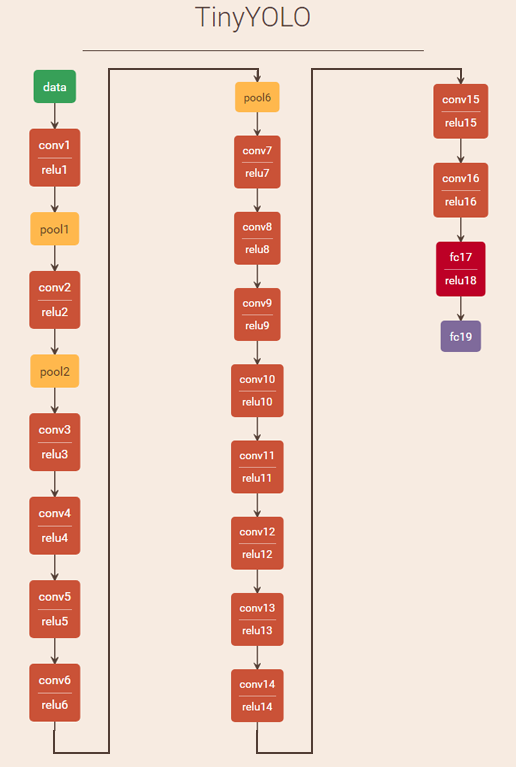
\includegraphics[width=0.75\linewidth]{tinyyoloar.png}
\end{center}
\end{figure}
\end{document}
\grid
